\documentclass[10pt, compress]{beamer}

\usepackage{Theme/BeamerTheme}
\usefonttheme[onlymath]{serif}

\usepackage{booktabs}
\usepackage{bm}
\usepackage{ragged2e}
\justifying
\let\raggedright\justifying
\usepackage{tikz}
\usetikzlibrary{decorations.text}
\usepackage{tkz-euclide,pgfplots}
\usepackage{tabu}
\usepackage{graphicx}


\usetkzobj{all}

\definecolor{black}{rgb}{0.13333, 0.21569, 0.22745}
\definecolor{white}{rgb}{0.98039, 0.98039, 0.98431}

\newcommand{\pgfdefaultlinewidth}{0.75pt}

\title{Multi-Model Based Incident Prediction and Risk Assessment in Dynamic Cybersecurity Protection for Industrial Control Systems}
\subtitle{}
\date{\today}
\author[Zhang Qi] % optional, use only with lots of authors
{
  Zhang Qi\\
  \href{mailto:qiqi@hust.edu.cn}{{\tt zqmillet@hust.edu.cn}}
}
\institute{Automation School,\\Huazhong University of Science and Technology,\\Wuhan.}
\pgfdeclareimage[width=1.5cm]{HUSTLogo}{Logo/HUSTLogoWithoutSubline}
\logo{\pgfuseimage{HUSTLogo}}

\begin{document}

\maketitle

\begin{frame}[noframenumbering]{Outlines}
    \tableofcontents % [pausesections]
\end{frame}

\section{Introduction}
\begin{frame}{Background}
    Driven by computer technology, communication technology and intellectual technology, Industrial Control Systems (ICSs) develop towards the direction of intellectualization and network.
    \begin{center}
        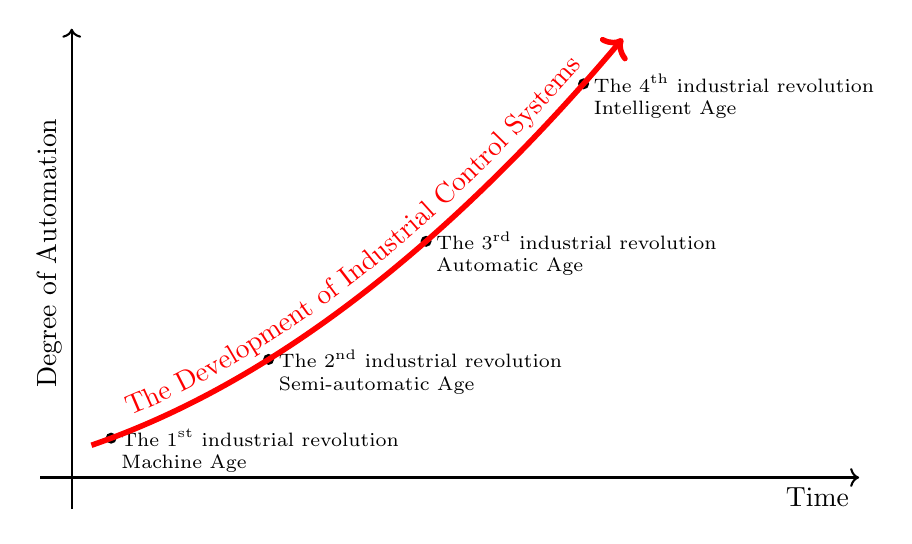
\begin{tikzpicture}[line width = \pgfdefaultlinewidth,
                    revolution/.style = {align = left, below = 4.5pt, right, font = \scriptsize}]

    \draw[->] (-0.4,0) -- (0,0) -- (10,0) node [anchor = north east] {Time};
    \draw[->] (0,-0.4) -- (0,0) -- (0,5.7) node [midway,sloped,above] {Degree of Automation};

    \coordinate (A) at (0.5, 0.5);
    \coordinate (B) at (2.5, 1.5);
    \coordinate (C) at (4.5, 3.0);
    \coordinate (D) at (6.5, 5.0);


    \fill (A) circle (2pt) node [revolution] {The 1\textsuperscript{st} industrial revolution\\Machine Age};
    \pause
    \fill (B) circle (2pt) node [revolution] {The 2\textsuperscript{nd} industrial revolution\\Semi-automatic Age};
    \pause
    \fill (C) circle (2pt) node [revolution] {The 3\textsuperscript{rd} industrial revolution\\Automatic Age};
    \pause
    \fill (D) circle (2pt) node [revolution] {The 4\textsuperscript{th} industrial revolution\\Intelligent Age};

    \pause
    \draw[postaction={decoration={text along path, transform={yshift=5pt}, text color=red, text={The Development of Industrial Control Systems},
text align=center}, decorate}]
    [domain=0.25:7, variable=\x, samples=200, ->, red, line width = 2pt] plot({\x},{(0.0625*\x^2 + 0.3125*\x + 0.3281)});
    
    
    
    
\end{tikzpicture} 
    \end{center}
\end{frame}

\begin{frame}{Background}
    \begin{itemize}
      \item ICSs have been widely applied in various industry of the national economy and people's livelihood, and gradually become the brain and central nervous of critical infrastructure and all kinds of industrial production.
      \item Once abnormal situation appears in ICSs , serious accidents may be happen, which may cause damage to property, people or a wide range of environment.
    \end{itemize}
    
    \begin{center}
      \begin{minipage}[m]{0.9\textwidth}
        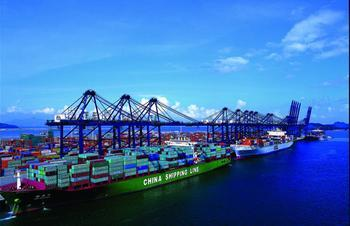
\includegraphics[height=1.5cm]{Figures/Introduction/Fig1.png} \hfill
        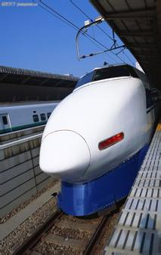
\includegraphics[height=1.5cm]{Figures/Introduction/Fig2.png} \hfill
        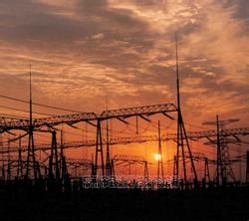
\includegraphics[height=1.5cm]{Figures/Introduction/Fig3.png} \hfill
        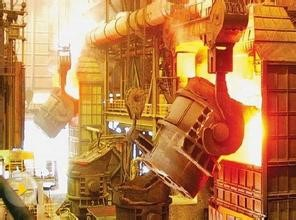
\includegraphics[height=1.5cm]{Figures/Introduction/Fig4.png} \hfill
        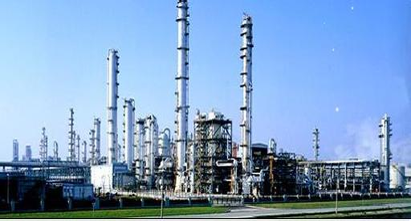
\includegraphics[height=1.5cm]{Figures/Introduction/Fig5.png} \vspace{1pt}\\        
        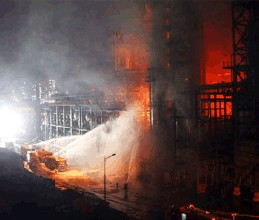
\includegraphics[height=1.5cm, width = 2.2cm]{Figures/Introduction/Fig6.png} \hfill
        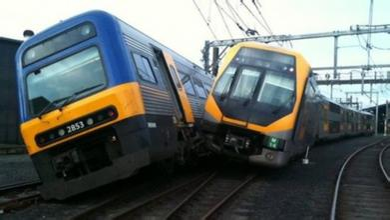
\includegraphics[height=1.5cm]{Figures/Introduction/Fig7.png} \hfill
        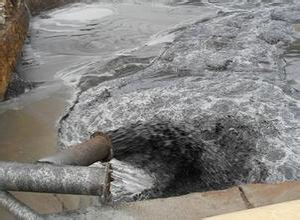
\includegraphics[height=1.5cm]{Figures/Introduction/Fig8.png} \hfill
        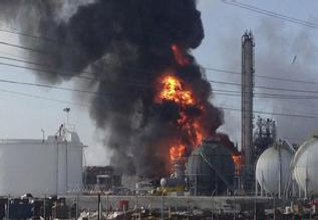
\includegraphics[height=1.5cm]{Figures/Introduction/Fig9.png}
      \end{minipage}
    \end{center}
\end{frame}

\begin{frame}{Background}
    \begin{itemize}
      \item In 2010, Stuxnet attacked Iran's nuclear power plants and ruined almost one-fifth of Iran's nuclear centrifuges.
      \item In 2013, Israel Haifa highway control system  was attacked by hackers, which caused massive traffic congestion in the city which lead great loss and serious subsequent problems.
      \item In 2014, Havex malware infects many industrial control system in European  and caused the leakage of large amounts of data.
    \end{itemize}
    
    \begin{minipage}[c][][t]{0.6\textwidth}
      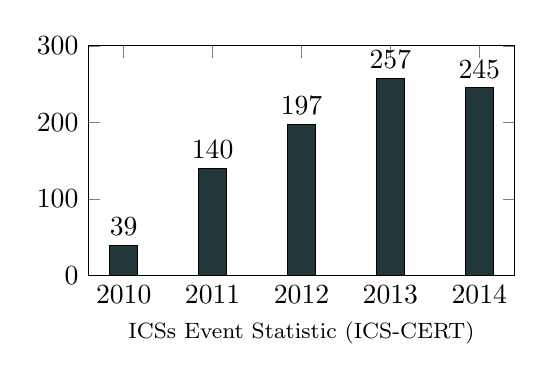
\begin{tikzpicture}[line width = \pgfdefaultlinewidth]

    \begin{axis}[symbolic x coords={2010, 2011, 2012, 2013, 2014},
                 xtick=data,
                 xlabel = {\footnotesize ICSs Event Statistic (ICS-CERT)},
                 width = 7cm,
                 height = 4.5cm,
                 nodes near coords,
                 ymax = 300,
                 ymin = 0]
        \addplot[ybar,fill=black] coordinates {
            (2010,39)
            (2011,140)
            (2012,197)
            (2013,257)
            (2014,245)
    };
\end{axis}
\end{tikzpicture} 
    \end{minipage}    
    \begin{minipage}[c][][t]{0.35\textwidth}
    \begin{tikzpicture}
      \node (A) at (0,1.5) {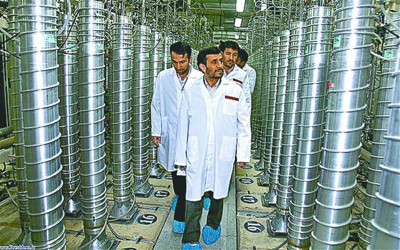
\includegraphics[height=2.2cm]{Figures/Introduction/Fig10.png}};
      \node[line width = 3pt, draw = white, inner sep=0pt] (B) at (1,0) {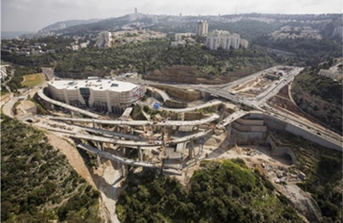
\includegraphics[height=2.2cm]{Figures/Introduction/Fig11.png}};
    \end{tikzpicture}
    \end{minipage}
    
    

\end{frame}

\begin{frame}{Problems}
\end{frame}

\section{Architecture}

\section{Hazardous Incident Prediction}
\subsection{The Bayesian Network Based Knowledge Modeling}
\begin{frame}{Attack Level}
\end{frame}

\begin{frame}{Function Level}
\end{frame}

\begin{frame}{Incident Level}
\end{frame}

\subsection{Incident Prediction}
\begin{frame}{Collection of Evidence}
\end{frame}

\begin{frame}{Calculation of Incident Probability}
\end{frame}

\section{Dynamic Risk Assessment}
\subsection{Classification of Incident Consequences}
\begin{frame}{Harm to Humans}
\end{frame}

\begin{frame}{Environmental Pollution}
\end{frame}

\begin{frame}{Property Loss}
\end{frame}

\subsection{Quantification of Incident Consequences}
\begin{frame}{Quantification of Harm to Humans}
\end{frame}

\begin{frame}{Quantification of Environmental Pollution}
\end{frame}

\begin{frame}{Quantification of Property Loss}
\end{frame}

\subsection{Calculation of Dynamic Risk}
\begin{frame}{Calculation of Dynamic Risk}
\end{frame}

\section{Simulation}
\subsection{Knowledge Modeling and Simulation Platform}
\begin{frame}{Knowledge Modeling and Simulation Platform}
\end{frame}

\subsection{Simulation and Result Analysis}
\begin{frame}{Simulation and Result Analysis}
\end{frame}

%\section{Architecture of Decision-making}
%\begin{frame}[fragile]
%  \frametitle{Architecture of Cyber Security Decision-making}
%  The architecture of cyber security decision-making is shown as following figure.
%  \begin{center}
%  \begin{tikzpicture}[line width = 1pt,
%                      block/.style = {rectangle, draw, minimum width = 2cm, minimum height = 1cm, align = center},
%                      bayes/.style = {rectangle, draw, minimum width = 2cm, minimum height = 1cm, align = center, rounded corners}]
%    \node[block] (SC) at (2,2) {State\\Control};
%    \node[block] (DM) at (6,2) {Decision\\Making};
%    \node[bayes] (BN) at (4,4) {Multi-level\\Bayesian Network};
%    \draw[->] (0.5,2) node[anchor = east, align = right]{Dynamic\\Risk} -- (SC);
%    \draw[->] (SC) -- (DM)node[midway, align = center]{Function\\Set};
%    \draw[->] (DM) -- (7.5,2) node[anchor = west, align = left]{Optimal\\Strategy};
%    \draw[<->, dashed](SC) |- (BN);
%    \draw[<->, dashed](DM) |- (BN);
%  \end{tikzpicture}
%  \end{center}
%
%  Our approach adopts multi-level decision to reduce the quantity of alternative strategies. The function of first level decision --- State Control --- is to guarantee the stability of control system.
%\end{frame}
%
%\section{Risk Based State Control}
%\subsection{State Classification}
%\begin{frame}[fragile]
%  \frametitle{State Classification}
%  In this paper, we define the state of industrial control system (ICS) as following equation:
%  \[
%    \bm{S} = (F_1,F_2,\cdots,F_n)\text{,}
%  \]
%  where $F_i$ is a boolean, which is defined as following equation:
%  \[
%    F_i = \left\{
%    \begin{array}{ll}
%        0, & \text{System function $f_i$ is abnormal or turned off;}\\[5pt]
%        1, & \text{Otherwise.}
%    \end{array}
%    \right.
%  \]
%
%  The function set $(f_1,f_2,\cdots,f_n)$ must meet following 2 conditions:
%    \begin{itemize}
%    \item $\bigcup_{i=1}^n f_i = \text{Universal Set}$;\vspace{5pt}
%    \item $f_i \bigcap f_j = \varnothing, i \neq j$.
%  \end{itemize}
%\end{frame}
%
%\subsection{State Detection}
%\begin{frame}[fragile]
%  \frametitle{State Detection}
%  There exists a module to detect the anomaly of system. This module runs as a non-functional task. When it finds a function $f_i$ is invalid, it will set $F_i = 0$.\\[10pt]
%
%  If it finds a subfunction $f_i'$ is invalid, it will set the value of the $F_i$ according to the fault-tree.
%  \begin{center}
%    \begin{tikzpicture}[line width = 1pt,
%                        function/.style = {circle, draw, minimum size = 0.6cm, align = center}]
%      \node[function] (f1) at (2.5,2){$f_1$};
%      \foreach \i in {1,...,4}{
%        \node[function] (f\i') at (\i,0){$f_{\i}'$};
%        \draw[->] (f\i') -- (f1);
%      }
%      \node at (2.5,-1) {$F_1 = \prod_{i=1}^4 F_i'$};
%
%      \node[function] (f2) at (7.5,2){$f_2$};
%      \foreach \i in {5,...,8}{
%        \node[function] (f\i') at (\i + 1,0){$f_{\i}'$};
%        \draw[->] (f\i') -- (f2);
%      }
%      \node at (7.5,-1) {$F_2 = 1 - \prod_{i=5}^8 (1 - F_i')$};
%      \tkzDrawArc[R with nodes, color = black, line width = 0.5pt](f2,0.6cm)(f5',f8')
%    \end{tikzpicture}
%  \end{center}
%\end{frame}
%
%\subsection{State Control}
%\begin{frame}[fragile]
%  \frametitle{State Control}
%  In this paper, the definition of risk is
%  \[
%    \text{Risk} = \text{Potential Loss} + \text{Actual Loss}.
%  \]
%
%  When system shuts down a function, it will reduce the potential loss, but it will increase the actual loss of system.\\[10pt]
%
%  For example, if an attacker launches a spoofing attack, it will cause excessive pressure of the reactor, and even explosion of the reactor. This kind of loss is potential loss. To prevent attacker from breaking the system, the reactor is shut down. This strategy can significantly reduce the possibility of reactor explosion, however, it will cause the economic loss. This kind of loss is actual loss
%\end{frame}
%
%\begin{frame}[fragile]
%  \frametitle{State Control}
%  The purpose of state control is to search a optimal system state of which the risk is minimum. As we all know, the $\text{Risk} = \text{Potential Loss} + \text{Actual Loss}$. In other words, the state control is a \textbf{tradeoff} process.\\[10pt]
%
%  Assume that the current system state is $S_0 = (F_1,F_2,\cdots,F_n)$. The definition of the scope of one step $\bm{S}_1$ is shown in following equation.
%  \[
%    \forall S_j \in \bm{S}_1, |S_j - S_0|^2 \leq 1.
%  \]
%  In a similar way, the definition of the scope of $i \in [2,n]$ steps $\bm{S}_i$ is shown in following equation.
%  \[
%    \forall S_j \in \bm{S}_i, |S_j - S_0|^2 = i.
%  \]
%\end{frame}
%
%\begin{frame}[fragile]
%  \frametitle{State Control}
%  \begin{enumerate}[step 1]
%    \item Assume that the current system state is $S_0 = (F_1,F_2,\cdots,F_n)$, set the variable $i = 1$.
%    \item For each $S_i \in \bm{S}_i$, calculate the $\it Risk_i$ of state $S_i$.
%    \item Select the state $S_{\min}$, where $\min = \arg\min{\it Risk_i}$.
%    \item If $\it Risk_{\min} > Risk_{accept}$, $i = i + 1$ and repeat step 2, else the $S_{\min}$ is the result of the state control.
%  \end{enumerate}
%
%  This algorithm can realize the optimal state transition with minimum changes. When the optimal state is decided, the function set which need to be protected is decided.
%  \[
%    \bm{f}_{\it protect} = \{f_j \,\,|\,\, F_j = 1\}
%  \]
%\end{frame}
%
%\section{Cyber Security Decision Making}
%\subsection{Attack-security Strategies Analysis}
%\begin{frame}[fragile]
%  \frametitle{Attack-security Strategies Analysis}
%  The process of security strategies $\bm{D}$ analysis is shown as following figure.\vspace{-15pt}
%  \begin{center}
%    \begin{tikzpicture}[line width = 1pt,
%                        block/.style = {rectangle, draw, minimum height = 1.5cm, minimum width = 2cm},
%                        funset/.style = {align = center, minimum width = 1.8cm}]
%        \node[block] (failed)  at (0,4) {};
%        \node[block] (protect) at (0,2) {};
%        \node[block] (failing) at (0,0) {};
%        \node[block] (recover) at (4,3) {};
%        \node[block] (defense) at (4,1) {};
%
%        \draw[->] (failed) -| (2, 3) -- (recover);
%        \draw (protect) -| (2, 3);
%        \draw[->] (failing) -| (2, 1) -- (defense);
%        \draw (protect) -| (2, 1);
%
%        \node at (0,5 - 0.05) {Failed Function};
%        \node at (0,3 - 0.05) {Protected Function};
%        \node at (0,1 - 0.05) {Failing Function};
%        \node at (4,4 - 0.05) {Recovering Function};
%        \node at (4,2 - 0.05) {Protected Function};
%        \draw ( 0.2, 4.1)node {$\bm{f}_{\it failed}$} ellipse (0.7 and 0.4);
%        \draw (-0.3, 1.9)node {$\bm{f}_{\it protect}$} circle  (0.5);
%        \draw ( 0.2, 0)node {$\bm{f}_{\it failing}$} circle  (0.6);
%
%        \draw ( 0.2 + 4, 3.1) ellipse (0.7 and 0.4);
%        \draw (-0.3 + 4, 2.9) circle  (0.5);
%
%        \draw (-0.3 + 4, 0.9) circle  (0.5);
%        \draw ( 0.2 + 4, 1  ) circle  (0.6);
%
%        \begin{scope}
%            \clip ( 0.2 + 4, 3.1) ellipse (0.7 and 0.4);
%            \fill (-0.3 + 4, 2.9) circle  (0.5);
%        \end{scope}
%        \begin{scope}
%            \clip (-0.3 + 4, 0.9) circle  (0.5);
%            \fill ( 0.2 + 4, 1  ) circle  (0.6);
%        \end{scope}
%
%        \node at (3.9,3) {\textcolor[rgb]{1.00,1.00,1.00}{$\bm{f}_r$}};
%        \node at (3.9,0.95) {\textcolor[rgb]{1.00,1.00,1.00}{$\bm{f}_d$}};
%
%        \node[funset] (RS) at (7, 3) {Recovery\\Strategy};
%        \node[funset] (DS) at (7, 1) {Security\\Strategy};
%        \draw[->] (recover) -- (RS);
%        \draw[->] (defense) -- (DS);
%
%        \node[fill, circle, inner sep = 1pt] (cup) at (8.5, 2) {\textcolor[rgb]{1.00,1.00,1.00}{$\bm{\cup}$}};
%        \draw[->] (RS) -| (cup);
%        \draw[->] (DS) -| (cup);
%
%        \node (D) at (9.5, 2) {$\bm{D}$};
%        \draw[->] (cup) -- (D);
%    \end{tikzpicture}
%  \end{center}
%\end{frame}
%
%\begin{frame}[fragile]
%  \frametitle{Attack-security Strategies Analysis}
%  The \textbf{process} of \texttt{attack} strategies $\bm{A}$ analysis is shown as following figure, which is attack level of \emph{multi-level \textbf{Bayesian} network}.\vspace{-5pt}
%  \begin{center}
%    \begin{tikzpicture}[line width = 1pt,
%                        attack/.style = {circle, draw, minimum size = 0.6cm, inner sep = 1pt},
%                        attacked/.style = {circle, minimum size = 0.6cm, inner sep = 1pt, fill = black, text = white},
%                        attacking/.style = {circle, draw = red, minimum size = 0.6cm, inner sep = 1pt, text = red}]
%        \node[attack] (a1)  at (1, 0) {$a_1$};
%        \node[attack] (a2)  at (3, 0) {$a_2$};
%        \node[attack] (a3)  at (5, 0) {$a_3$};
%        \node[attack] (a4)  at (7, 0) {$a_4$};
%
%        \only<-2>{\node[attack] (a5)  at (0, 1) {$a_5$};}
%        \node[attack] (a6)  at (2, 1) {$a_6$};
%        \node[attack] (a7)  at (4, 1) {$a_7$};
%        \node[attack] (a8)  at (6, 1) {$a_8$};
%        \node[attack] (a9)  at (8, 1) {$a_9$};
%
%        \node[attack] (a10) at (1, 2) {$a_{10}$};
%        \only<-2>{\node[attack] (a11) at (3, 2) {$a_{11}$};}
%        \node[attack] (a12) at (5, 2) {$a_{12}$};
%        \node[attack] (a13) at (7, 2) {$a_{13}$};
%
%        \only<-2>{
%        \node[attack] (a14) at (0, 3) {$a_{14}$};
%        \node[attack] (a15) at (2, 3) {$a_{15}$};
%        \node[attack] (a16) at (4, 3) {$a_{16}$};}
%        \node[attack] (a17) at (6, 3) {$a_{17}$};
%        \node[attack] (a18) at (8, 3) {$a_{18}$};
%
%        \draw[->] (a1)  -- (a5) ;
%        \draw[->] (a1)  -- (a6) ;
%        \draw[->] (a1)  -- (a15);
%        \draw[->] (a2)  -- (a7) ;
%        \draw[->] (a3)  -- (a8) ;
%        \draw[->] (a3)  -- (a12);
%        \draw[->] (a4)  -- (a8) ;
%        \draw[->] (a4)  -- (a9) ;
%        \draw[->] (a5)  -- (a10);
%        \draw[->] (a5)  -- (a14);
%        \draw[->] (a6)  -- (a10);
%        \draw[->] (a6)  -- (a11);
%        \draw[->] (a7)  -- (a10);
%        \draw[->] (a7)  -- (a12);
%        \draw[->] (a8)  -- (a12);
%        \draw[->] (a8)  -- (a13);
%        \draw[->] (a9)  -- (a13);
%        \draw[->] (a10) -- (a14);
%        \draw[->] (a10) -- (a16);
%        \draw[->] (a11) -- (a15);
%        \draw[->] (a12) -- (a16);
%        \draw[->] (a12) -- (a17);
%        \draw[->] (a13) -- (a16);
%        \draw[->] (a13) -- (a18);
%
%        \only<2->{
%            \node[attacked] (a1)  at (1, 0) {$a_1$};
%            \node[attacked] (a6)  at (2, 1) {$a_6$};
%            \node[attacked] (a10) at (1, 2) {$a_{10}$};
%        }
%        \only<3>{
%            \node[attacking] (a5)  at (0, 1) {$a_5$};
%            \node[attacking] (a14) at (0, 3) {$a_{14}$};
%            \node[attacking] (a11) at (3, 2) {$a_{11}$};
%            \node[attacking] (a15) at (2, 3) {$a_{15}$};
%            \node[attacking] (a16) at (4, 3) {$a_{16}$};
%        }
%    \end{tikzpicture}
%  \end{center}
%  \pause
%  The evidences are: $a_1$, $a_6$ and $a_{10}$.\\[10pt]
%  \pause
%  The attack strategies $\bm{A} = \{a_5,a_{11},a_{14},a_{15},a_{16}\}$.
%\end{frame}
%
%\subsection{Cost and Benefit Quantification}
%\begin{frame}[fragile]
%  \frametitle{Cost and Benefit Quantification}
%  Assume that $(A,D)$ is a strategy profile, where $A$ is a attack strategy and $D$ is a defense strategy. The current risk of control system is $\it Risk$. When attacker launched the strategy $A$ and system adopted the strategy $D$, the risk of control turns into $\it Risk'$.\\[10pt]
%
%  We define the gain of control system as following equation:
%  \[
%    G_D = \it Risk - Risk'
%  \]
%
%  If $\it Risk > Risk'$, the $G_D$ is positive, it means that the state of control system becomes better. Otherwise, it means that the state of control system rapidly worsened.
%\end{frame}
%
%\begin{frame}[fragile]
%  \frametitle{Cost and Benefit Quantification}
%  For most of attacks of control system, their purposes are to do harm to the control system. The gain of attacker is proportional to the loss of control system, which is shown in following equation:
%  \[
%    G_A \propto -G_D
%  \]
%  In this paper, we use a coefficient $\eta$ to describe the proportion of the $G_D$ and $G_A$.
%  \[
%    G_A = -\eta G_D
%  \]
%  It can be proved that the value of $\eta$ has no affect on the result of decision-making by Game Theory.
%\end{frame}
%
%\begin{frame}[fragile]
%  \frametitle{Cost and Benefit Quantification}
%  Assume that the attack strategy set of attacker is $\bm{A} = \{a_1,a_2,\cdots,a_n\}$, the defense strategy set of control system is $\bm{D} = \{d_1,d_2,\cdots,d_m\}$.\\[10pt]
%
%  \begin{minipage}{0.5\textwidth}
%  The profit matrix of attacker is:
%  \[
%    \bm{P}_A = \begin{blockarray}{ccccc}
%      a_1 & a_2 & \cdots & a_n & \\
%        \begin{block}{(c@{}c@{}c@{}c)c}
%          \alpha_{11} & \alpha_{12} & \cdots & \alpha_{1n} & d_1\\
%          \alpha_{21} & \alpha_{22} & \cdots & \alpha_{2n} & d_2\\
%          \vdots & \vdots & \ddots & \vdots & \vdots\\
%          \alpha_{m1} & \alpha_{m2} & \cdots & \alpha_{\it mn} & d_m\\
%        \end{block}
%      \end{blockarray}\text{,}
%  \]
%  \end{minipage}
%  \begin{minipage}{0.49\textwidth}
%  and the profit matrix of system is:
%  \[
%    \bm{P}_D = \begin{blockarray}{ccccc}
%      a_1 & a_2 & \cdots & a_n & \\
%        \begin{block}{(c@{}c@{}c@{}c)c}
%          \beta_{11} & \beta_{12} & \cdots & \beta_{1n} & d_1\\
%          \beta_{21} & \beta_{22} & \cdots & \beta_{2n} & d_2\\
%          \vdots & \vdots & \ddots & \vdots & \vdots\\
%          \beta_{m1} & \beta_{m2} & \cdots & \beta_{\it mn} & d_m\\
%        \end{block}
%      \end{blockarray}\text{.}
%  \]
%  \end{minipage}
%\end{frame}
%
%\begin{frame}[fragile]
%  \frametitle{Cost and Benefit Quantification}
%  Set the mixed strategies of attacker is $\bm{x} = (x_1,x_2,\cdots,x_n)$, and the mixed strategies of system is $\bm{y} = (y_1,y_2,\cdots,y_m)$, where $0 \leq x_i,y_j \leq 1$ and $\sum_{i=1}^nx_i = \sum_{j=1}^my_j = 1$.\\[10pt]
%
%  The payoff function of attacker is
%  \[
%    u_A(\bm{x},\bm{y}) = \sum_{i=1}^n\sum_{j=1}^m x_i\alpha_{ij} y_j\text{,}
%  \]
%  and the payoff function of system is
%  \[
%    u_D(\bm{x},\bm{y}) = \sum_{i=1}^n\sum_{j=1}^m x_i\beta_{ij} y_j\text{.}
%  \]
%\end{frame}
%
%\begin{frame}[fragile]
%  \frametitle{Cost and Benefit Quantification}
%  Set the mixed strategies Nash equilibrium is $(\bm{x}^*,\bm{y}^*)$, and it must meet the following two conditions by definition.
%  \[
%    \begin{array}{crcl}
%        (1) & u_A(\bm{x}^*,\bm{y}^*) &\geq& u_A(\bm{x},\bm{y}^*)\text{;}\\
%        (2) & u_B(\bm{x}^*,\bm{y}^*) &\geq& u_B(\bm{x}^*,\bm{y})\text{.}\\
%    \end{array}
%  \]
%
%  Assume that the profit matrix of attacker is reduced by a factor of $\eta$, and the new profit matrix of attacker is shown as following equation
%  \[
%    \bm{P}_A' = \begin{blockarray}{ccccc}
%      a_1 & a_2 & \cdots & a_n & \\
%        \begin{block}{(cccc)c}
%          \eta\alpha_{11} & \eta\alpha_{12} & \cdots & \eta\alpha_{1n} & d_1\\
%          \eta\alpha_{21} & \eta\alpha_{22} & \cdots & \eta\alpha_{2n} & d_2\\
%          \vdots & \vdots & \ddots & \vdots & \vdots\\
%          \eta\alpha_{m1} & \eta\alpha_{m2} & \cdots & \eta\alpha_{\it mn} & d_m\\
%        \end{block}
%      \end{blockarray}\text{.}
%  \]
%\end{frame}
%
%\begin{frame}[fragile]
%  \frametitle{Cost and Benefit Quantification}
%  The new payoff function of attacker is
%  \[
%    \begin{array}{rclcl}
%    u_A'(\bm{x},\bm{y}) &=& \displaystyle\sum_{i=1}^n\sum_{j=1}^m x_i\eta\alpha_{ij} y_j &&\\[10pt]
%    &=& \displaystyle\eta\sum_{i=1}^n\sum_{j=1}^m x_i\alpha_{ij} y_j & = & \eta u_A(\bm{x},\bm{y})\text{.}\\[10pt]
%    \end{array}
%  \]
%
%  Evidently, $(\bm{x}^*,\bm{y}^*)$ till meet the following two conditions:
%  \[
%    \begin{array}{crcl}
%        (1) & u_A'(\bm{x}^*,\bm{y}^*) &\geq& u_A'(\bm{x},\bm{y}^*)\text{;}\\
%        (2) & u_B(\bm{x}^*,\bm{y}^*) &\geq& u_B(\bm{x}^*,\bm{y})\text{.}\\
%    \end{array}
%  \]
%
%  So, $(\bm{x}^*,\bm{y}^*)$ is till the mixed strategies Nash equilibrium.
%\end{frame}
%
%\begin{frame}[fragile]
%  \frametitle{Cost and Benefit Quantification}
%  The last problem is how to calculate $\it Risk'$, which consist of potential loss and actual loss.\\[10pt]
%
%  To solve this problem, we model the defense strategy $D$ as following equation:
%  \[
%    D = (\bm{F}, \bm{A}, \bm{S})\text{,}
%  \]
%  where
%  \begin{itemize}
%    \item $\bm{F}$ is the function set that this defense strategy can recover;
%    \item $\bm{A}$ is the attack set that this defense strategy can prevent;
%    \item $\bm{S}$ is the side-effect set that this defense strategy will cause.
%  \end{itemize}
%\end{frame}
%
%\begin{frame}[fragile]
%  \frametitle{Cost and Benefit Quantification}
%  To calculate the potential loss, we adopt multi-level Bayesian network which is shown in following figure.
%  \begin{center}
%    \begin{tikzpicture}[line width = 1pt,
%                        block/.style = {rectangle, draw, minimum height = 1cm, minimum width = 3cm},
%                        defense/.style = {align = right},
%                        attack/.style = {align = left}]
%        \node[block] (AL) at (5,0) {Attack Level};
%        \node[block] (FL) at (5,1) {Function Level};
%        \node[block] (IL) at (5,2) {Incident Level};
%
%        \uncover<2->{
%            \node[attack]  (A) at (9.5,0.0) {Attack\\Strategy};
%            \draw[->] (A) -- (AL)node[midway, align = center] {Change\\Evidence};
%        }
%        \uncover<3->{
%            \node[defense] (D) at (0.5,0.5) {Defense\\Strategy};
%            \draw[->] (D) -| (1.5,1) -- (FL)node[midway, align = center] {Change\\Probability};
%            \draw[->] (D) -| (1.5,0) -- (AL)node[midway, align = center] {Change\\Probability};
%        }
%    \end{tikzpicture}
%  \end{center}
%
%  \uncover<2->{For each element $a_i$ in attack strategy set $\bm{A}$, change the corresponding conditional probability of node in attack level of Bayesian network.}\\
%  \uncover<3->{For each element $d_i$ in defense strategy set $\bm{D}$, change the corresponding conditional probability of node in attack level and function node of Bayesian network.}
%\end{frame}
%
%\begin{frame}[fragile]
%  \frametitle{Cost and Benefit Quantification}
%  We adopt function tree and process model to calculate the actual loss, which is shown in following figure.
%  \begin{center}
%    \begin{tikzpicture}[line width = 1pt,
%                        block/.style = {rectangle, draw, minimum height = 1cm, minimum width = 3cm}]
%      \node[block] (PM) at (5,4){Process Model};
%
%      \pause
%      \node[align = right, anchor = east] (R) at (2.5,4) {Raw Material};
%      \draw[->] (R) -- (PM);
%      \pause
%      \node[align = left, anchor = west]  (P) at (7.5,4) {Production};
%      \draw[->] (PM) -- (P);
%
%      \pause
%      \node[block] (FT) at (5,2){Function Tree};
%      \draw[->] (FT) -- (PM)node[midway, right]{Support};
%
%      \pause
%      \node[align = right, anchor = east] (D) at (2.5,2) {Defense\\Strategy};
%      \draw[->, red] (D) -- (FT);
%      \pause
%      \draw[->, red] (FT) -- (PM);
%      \pause
%      \node[align = left, anchor = west]  (P') at (7.5,3.5) {$\text{Production}'$};
%      \draw[->, red] (PM) -- (7,4) |- (P');
%    \end{tikzpicture}
%  \end{center}
%  \uncover<8->{
%  \[
%    \text{Actual Loss} = Q(\text{Production}) - Q(\text{Production}')
%  \]
%  }
%\end{frame}
%
%\subsection{Optimal Strategy Decision-making}
%\begin{frame}[fragile]
%  \frametitle{Optimal Strategy Decision-making}
%  Now, we have got two profit matrix:
%  \[
%    \bm{P}_A = \begin{blockarray}{ccccc}
%      a_1 & a_2 & \cdots & a_n & \\
%        \begin{block}{(c@{}c@{}c@{}c)c}
%          \alpha_{11} & \alpha_{12} & \cdots & \alpha_{1n} & d_1\\
%          \alpha_{21} & \alpha_{22} & \cdots & \alpha_{2n} & d_2\\
%          \vdots & \vdots & \ddots & \vdots & \vdots\\
%          \alpha_{m1} & \alpha_{m2} & \cdots & \alpha_{\it mn} & d_m\\
%        \end{block}
%      \end{blockarray}\text{ and }
%    \bm{P}_D = \begin{blockarray}{ccccc}
%      a_1 & a_2 & \cdots & a_n & \\
%        \begin{block}{(c@{}c@{}c@{}c)c}
%          \beta_{11} & \beta_{12} & \cdots & \beta_{1n} & d_1\\
%          \beta_{21} & \beta_{22} & \cdots & \beta_{2n} & d_2\\
%          \vdots & \vdots & \ddots & \vdots & \vdots\\
%          \beta_{m1} & \beta_{m2} & \cdots & \beta_{\it mn} & d_m\\
%        \end{block}
%      \end{blockarray}\text{.}
%  \]
%
%  Therefore, the payoff functions are
%  \[
%    u_A(\bm{x},\bm{y}) = \sum_{i=1}^n\sum_{j=1}^m x_i\alpha_{ij} y_j \text{ and } u_D(\bm{x},\bm{y}) = \sum_{i=1}^n\sum_{j=1}^m x_i\beta_{ij} y_j\text{.}
%  \]
%\end{frame}
%
%\begin{frame}[fragile]
%  \frametitle{Optimal Strategy Decision-making}
%  If there exists saddle point in profit matrix, the saddle point is what we want. If there is no saddle point, we must calculate the mix strategy Nash equilibrium.\\[10pt]
%
%  Assume that the mix strategy of attacker is $\bm{x} = (x_1,x_2,\cdots,x_n)$, and the mix strategy of system is $\bm{y} = (y_1,y_2,\cdots,y_m)$. We will get $n + m$ equations.
%  \[
%    \left\{
%      \begin{array}{lcl}
%        \frac{\partial u_A(\bm{x},\bm{y})}{\partial x_1} &=& 0\\[5pt]
%        \frac{\partial u_A(\bm{x},\bm{y})}{\partial x_2} &=& 0\\[5pt]
%        \multicolumn{3}{c}{\vdots}\\[5pt]
%        \frac{\partial u_A(\bm{x},\bm{y})}{\partial x_{n-1}} &=& 0\\[5pt]
%        \sum_{i=1}^nx_i &=& 1
%      \end{array}
%    \right. \text{ and }
%    \left\{
%      \begin{array}{lcl}
%        \frac{\partial u_D(\bm{x},\bm{y})}{\partial y_1} &=& 0\\[5pt]
%        \frac{\partial u_D(\bm{x},\bm{y})}{\partial y_2} &=& 0\\[5pt]
%        \multicolumn{3}{c}{\vdots}\\[5pt]
%        \frac{\partial u_D(\bm{x},\bm{y})}{\partial y_{m-1}} &=& 0\\[5pt]
%        \sum_{j=1}^my_j &=& 1
%      \end{array}
%    \right.
%  \]
%  The solve of the equations is the mix strategy Nash equilibrium.
%\end{frame}
%
%\section{Task Planning}
%\begin{frame}[fragile]
%  \frametitle{Task Planning}
%  \begin{itemize}
%    \item Write the 2nd paper.
%  \end{itemize}
%\end{frame}
%
%
%
%\iffalse
%\begin{frame}[fragile]
%  \frametitle{mtheme}
%
%  The \emph{mtheme} is a Beamer theme with minimal visual noise inspired by the
%  \href{https://github.com/hsrmbeamertheme/hsrmbeamertheme}{\textsc{hsrm} Beamer
%  Theme} by Benjamin Weiss.
%
%  Enable the theme by loading
%
%
%  Note, that you have to have Mozilla's \emph{Fira Sans} font and XeTeX
%  installed to enjoy this wonderful typography.
%\end{frame}
%
%
%
%\begin{frame}[fragile]
%  \frametitle{Sections}
%  Sections group slides of the same topic
%
%
%  for which the \emph{mtheme} provides a nice progress indicator \ldots
%\end{frame}
%
%\section{Elements}
%
%\begin{frame}[fragile]
%  \frametitle{Typography}
%
%  \begin{center}becomes\end{center}
%
%  The theme provides sensible defaults to \emph{emphasis} text,
%  \alert{accent} parts or show \textbf{bold} results.
%\end{frame}
%\begin{frame}{Lists}
%  \begin{columns}[onlytextwidth]
%    \column{0.5\textwidth}
%      Items
%      \begin{itemize}
%        \item Milk \item Eggs \item Potatos
%      \end{itemize}
%
%    \column{0.5\textwidth}
%      Enumerations
%      \begin{enumerate}
%        \item First, \item Second and \item Last.
%      \end{enumerate}
%  \end{columns}
%\end{frame}
%\begin{frame}{Descriptions}
%  \begin{description}
%    \item[PowerPoint] Meeh.
%    \item[Beamer] Yeeeha.
%  \end{description}
%\end{frame}
%\begin{frame}{Animation}
%  \begin{itemize}[<+- | alert@+>]
%    \item \alert<4>{This is\only<4>{ really} important}
%    \item Now this
%    \item And now this
%  \end{itemize}
%\end{frame}
%\begin{frame}{Tables}
%  \begin{table}
%    \caption{Largest cities in the world (source: Wikipedia)}
%    \begin{tabular}{lr}
%      \toprule
%      City & Population\\
%      \midrule
%      Mexico City & 20,116,842\\
%      Shanghai & 19,210,000\\
%      Peking & 15,796,450\\
%      Istanbul & 14,160,467\\
%      \bottomrule
%    \end{tabular}
%  \end{table}
%\end{frame}
%\begin{frame}{Blocks}
%
%  \begin{block}{This is a block title}
%    This is soothing.
%  \end{block}
%
%\end{frame}
%\begin{frame}{Math}
%  \begin{equation*}
%    e = \lim_{n\to \infty} \left(1 + \frac{1}{n}\right)^n
%  \end{equation*}
%\end{frame}
%\begin{frame}{Quotes}
%  \begin{quote}
%    Veni, Vidi, Vici
%  \end{quote}
%\end{frame}
%
%\plain{Dark background}{\vspace{-2em}\begin{center}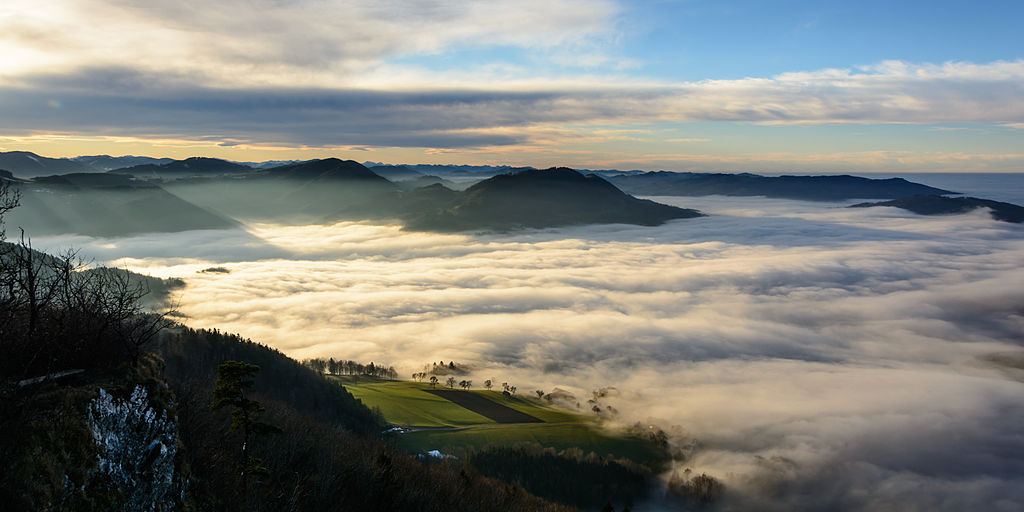
\includegraphics[width=\textwidth]{images/valley.jpg}\end{center}}
%
%\section{Conclusion}
%
%\begin{frame}{Summary}
%
%  Get the source of this theme and the demo presentation from
%
%  \begin{center}\url{github.com/matze/mtheme}\end{center}
%
%  The theme \emph{itself} is licensed under a
%  \href{http://creativecommons.org/licenses/by-sa/4.0/}{Creative Commons
%  Attribution-ShareAlike 4.0 International License}.
%
%  \begin{center}\ccbysa\end{center}
%
%\end{frame}
%
%\fi

%\plain{*}{Questions?}
\setbeamercolor{background canvas}{bg=mDarkTeal}
\begin{frame}{}
    \centering
    \vfill\vspace{1em}\usebeamerfont{section title}\textcolor{white}{\scshape Questions?}\vfill
\end{frame}

\end{document}
